\section{Client-server architecture}

\begin{figure}[H]
    \centering
    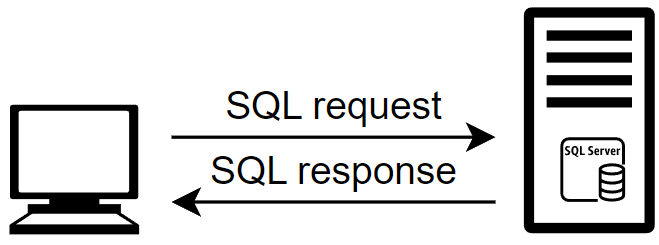
\includegraphics[width=0.25\linewidth]{images/cs.png}
\end{figure}

\paragraph*{Hardware}
In the client-server architecture, the hardware components consist of:
\begin{itemize}
    \item A server responsible for data management.
    \item A client handling presentation layout.
\end{itemize}

\paragraph*{Software}
The client software dispatches requests to the server through SQL queries and encompasses both business and presentation logic.
The server software is tasked with processing queries and responding by transmitting result sets back to the client and 
This software is dedicated to data management.

\paragraph*{Network}
The network topology is structured as a local area network comprising one or more servers and multiple clients.